\chapter[Capítulo 3]{Situação Atual e Desenvolvimento do Sistema de Design no TCE-RN}
\label{ch:cap3}

  Tendo em vista o potencial que ferramentas de design e prototipação possuem em acelerar o desenvolvimento e a validação sistemas e serviços e a necessidade do Tribunal de Contas do Estado em agilizar os seus processos de desenvolvimento e a crescente demanda de por novos sistemas e pela evolução dos sistemas e serviços prestados não somente a suas diretorias como aos entes jurisdicionados foi abordada junto a DIN se haveria por parte deles o interesse no desenvolvimento de um sistema de design. A Diretoria de Informatica se mostrou interessada e foi dado inicio o desenvolvolvimento do trabalho.

  Como visto anteriormente um sistema de design é um produto, que por sua vez tem a intenção de servir outros produtos, que seriam os sistemas desenvolvidos pela instituição baseados nas diretivas criadas por esse sistema, é de responabiliade do Sistema de Design (SD) possibilitar tanto a prototipação rápida, de baixa fidelidade, como a de alta fidelidade, assim como validar as evoluções feitas em sistemas preexistentes junto aos clientes. Sendo essas apenas algumas das responsabiliades desse produto.

\section{Situação Atual Do Design no TCE-RN} \label{secao31}
  A história do Tribunal de Contas do Estado começou oficialmente em 12 de janeiro de 1961, data oficial da sua criação \cite{historia_tribunal} O tribunal vem ao longo desses anos evoluindo sempre e gerenciando projetos cadas vez mais complexos, agregando as responsabilidades de fiscalização e divulgação dos pareceres do poder legislativo Municipal. Contudo do ponto de vista do design o TCE-RN avançou pouco nos ultimos anos. Apesar de possuir em suas politicas de desenvolvimento a obrigatoriedade da construção de um prototipo que precisa ser validado junto ao cliente que ira usar o software ou serviço, para saber se o mesmo tem suas necessidades atendidas essa prototipação atualmente é feita por meio da ferramenta de prototipação Pencil Project (Pencil) que possue varais limitações em relação a ferramentas de design mais modernas como demonstrado na tabela \ref{table-figma_vs_pencil} Vantagens Figma vs Pencil.

  Em 2019 o TCE-RN iniciou o desenvolvimento de uma nova biblioteca de componentes para construção de interfaces web. Essa biblioteca é construida sobre uma plataforma de desenvolvimento em Javascript chamada Angular, Javascript por sua vez é uma linguagem de Programação de proposito geral, multiparadigma que juntamente com as tecnologias HTML (HyperText Markup Language), uma lingaugem de marcação de hipertexto e CSS (Cascate Style Sheet), o mecanismo de acionamento de estilos de interpretadores web representam os 3 pilares fundamentais usados no desenvolvimento de sistemas web modernos.

  Para a construção do seu front-end, que são sistemas com a qual os usuários interagem diretamente, o tribunal usa tecnologias modernas e em constante evolução, contudo para a prototipação, o Pencil oferece poucas vantagens em relação a maioria das ferramentas citadas no Capítulo \ref{ch:cap2} como por exemplo testes de usabilidade ou a presença de animações ou transições que aproximem o usuario da experiencia final do uso do software em Desenvolvimento.

  \begin{table*}[!ht]
    \centering
    \caption{Vantagens Figma vs Pencil}
    \begin{tabular}{lll}
      
      \rowcolor[HTML]{AAAAAA}
      Caracteristicas             &
      Figma                       &
      Pencil                      \\
      \rowcolor[HTML]{DDDDDD}
      Facil de usar               &
      sim                         &
      sim                         \\
      Colaborativo                &
      sim                         &
      não                         \\
      \rowcolor[HTML]{DDDDDD}
      Animação                    &
      sim                         &
      não                         \\
      Arrastar e soltar           &
      sim                         &
      sim                         \\
      \rowcolor[HTML]{DDDDDD}
      Prototipo de Software       &
      sim                         &
      não                         \\
      Prototipação de Interfaces  &
      sim                         &
      sim                         \\
      \rowcolor[HTML]{DDDDDD}
      Prototipação de UX          &
      sim                         &
      não                         \\
      Teste de Usabilidade        &
      sim                         &
      não                         \\
      \rowcolor[HTML]{DDDDDD}
      Controle de Versao          &
      sim                         &
      não                         \\
    \end{tabular}
    \label{table-figma_vs_pencil}
    \fonte{\cite{figma_vs_pencil}}
  \end{table*}

  O fluxo de trabalho até o momento para o desenvolvimento de prototipos consiste em copiar um projeto preexistente e utilizar a maior quantidade possivel de elementos de layout desse documento do Pencil. No entando como foi dito anteriormente o tribunal passou a evoluir a biblioteca de componentes de front-end dos seus sistemas, e por não possuir um sistema de versionamento o Pencil não é capaz de refletir essas modificações. Tambem não é permitido que o usuario teste a o fluxo da experiência de uso dos sistemas com o usuário. Por esses e outros motivos como demonstrado na Tabela \ref{table-figma_vs_pencil} o Figma foi escolhido como ferramenta de desenvolvimento de sistema design para ser usado neste trabalho, que possui o intuito de trazer uma maneira mais dinamica de criar e testar as interfaces do TCE-RN e permitir que a todo sistema possa sofrer mudanças e evoluções mais suavemente de maneira concisa e consistente.

\section{Reconstrução Do Modelo Existente} \label{secao32}

  O ponto de partida foi recriar modelos dos elementos preexistentes nos layouts de sistemas do TCE-RN. Foram favorecidos os sistemas que implementacem a bibliteca de componentes recem desenvolvida em detrimento as demais pois estes expressam de maneira mais acurada as intenções do tribunal quanto a aparência e usabilidade a serem experimentadas pelos usuarios num futuro proximo.

  Executando uma instância de exemplo da biblioteca de componentes criadas em Angular e usando o navegador Brave foi possível utilizar uma das funcionalidades desse navegador, o CSS Overview, para inspecionar as caracteristicas do projeto e a situação atual da biblioteca, tornando possivel realizar o levantamento dos diferentes aspectos dos componentes como por exemplo a quantidade de cores diferentes presentes nas paginas, onde essas cores eram usadas, quais os códigos hexadecimais referente a cada cor, quantos e quais os breakpoints de tamanho das midias, e outras informações relevantes. Um exemplo de inspeção de pagina pode ser encontrao na figura \ref{fig:tcenglib} Analise da biblioteca de componentes existente no TCE-RN.

  \begin{figure}[!h]
    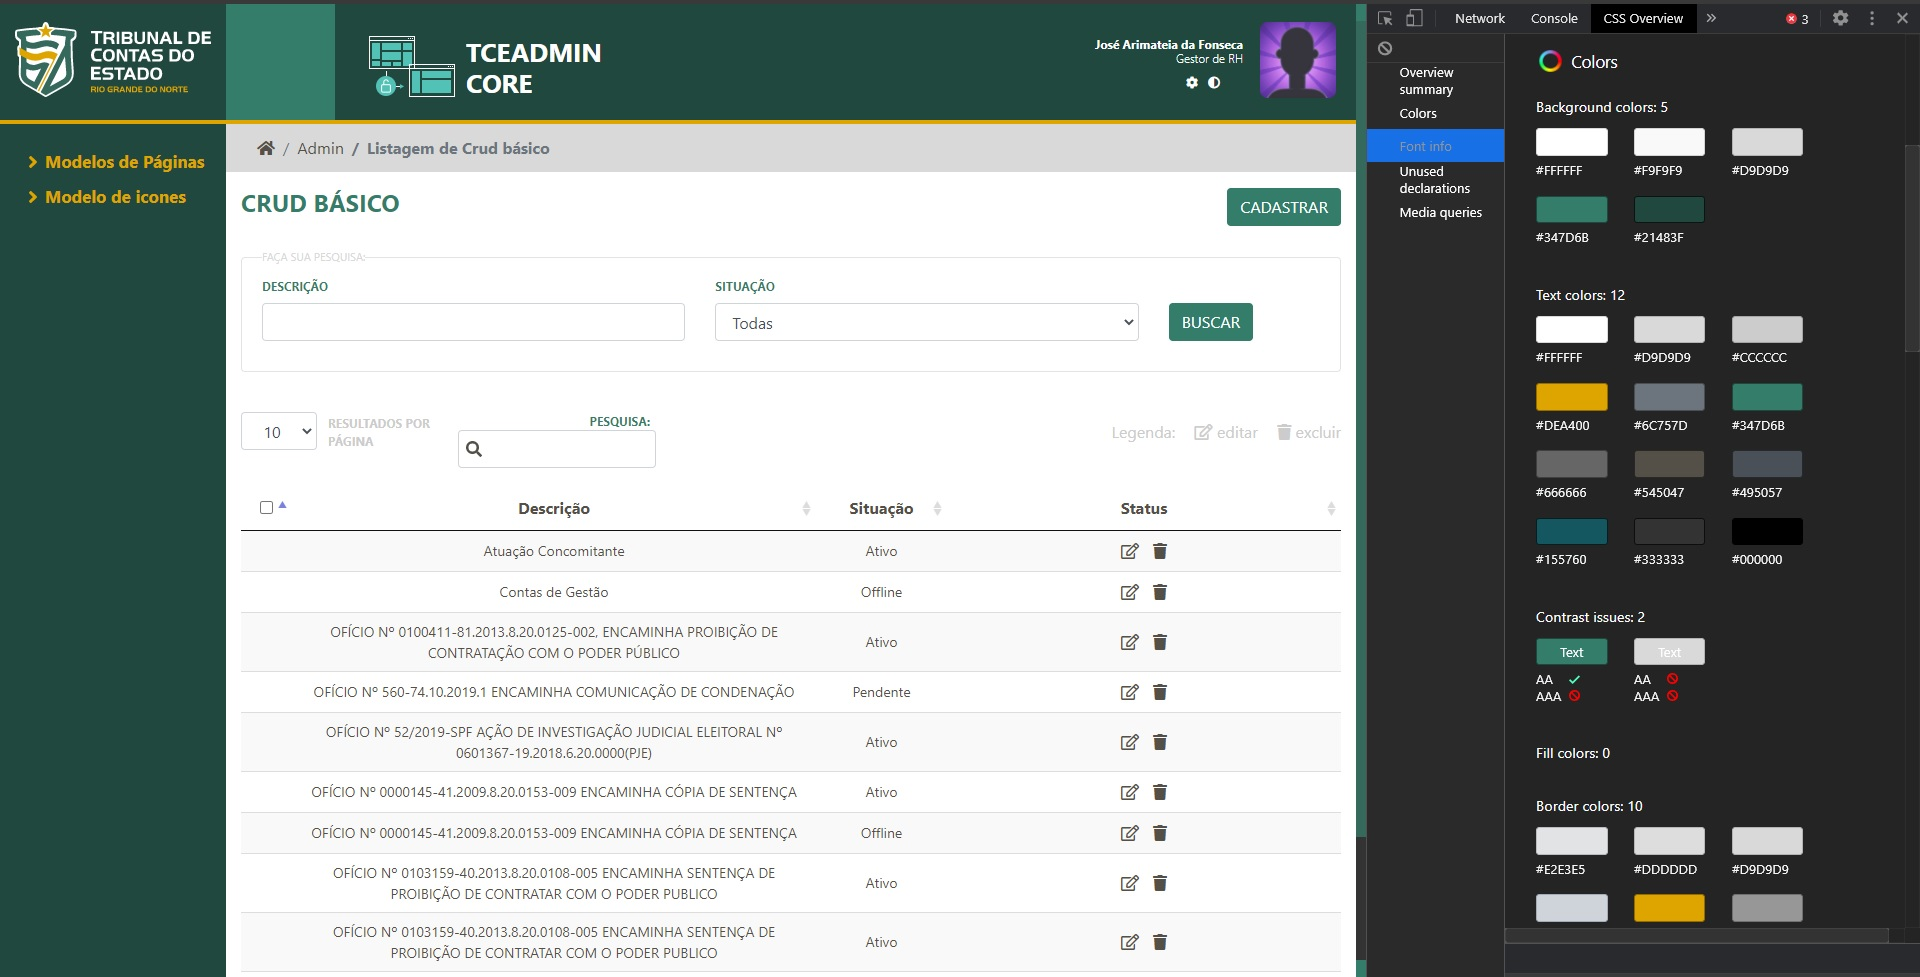
\includegraphics[width=\linewidth]{tce-lib.jpg}
    \caption{Analise da biblioteca de componentes existente no TCE-RN.}
    \label{fig:tcenglib}
  \end{figure}

  De posse dos elementos fundamentais que já estavam sendo usados em conjunto com as metricas que os mesmos possuiam o passo seguinte foi a construção dessa instância atual na ferramenta Figma proposta pelas vantagens citadas no Capitulo \ref{ch:cap2}. Em um primeiro momento foi utilizada a metodologia atomica de design para o desenvolvimento desse modelo inicial "In the natural world, atomic elements combine together to form molecules. These molecules can combine further to form relatively complex organisms" \cite{atomic_design}. Construir elementos mais complexos apartir de elementos mais simples associado a uma ação facilitada por uma funcionalidade do Figma de permitir a construção de "componentes mestres", estruturas das quais podem ser criadas instancias e que quando edições são realizadas no componente mestre as mesmas são herdadas para todos os elementos copiados apartir deste, o que permitiu reduzir a carga de trabalho, pois mudanças e melhorias nos elementos não precisavam ser replicadas em elementos acima da na construção hierarquica dos componentes.

  O intuito desta primeira abordagem era o de separar os elementos existentes em elementos mais fundamentais que pudessem ser identificados como reaproveitaveis por componentes com hierarquias e complexidades mais elevadas. Esta separação segue uma sequencia intuitiva de agrupamentos por atomos, moleculas e organismos, em que, atomos constituem os blocos fundamentais usados por moleculas, sendo estes estruturas um pouco mais complexas como por xemplo um campo de entrada de texto ou um botão, que por sua vez agrupados compõem organismos, estruturas ainda mais complexas que englobam multiplos atomos e moleculas. Um exemplo dessa Composição e reaproveitamento pode ser visto na figura \ref{fig:mastercomponent}

  \begin{figure}[h!]
    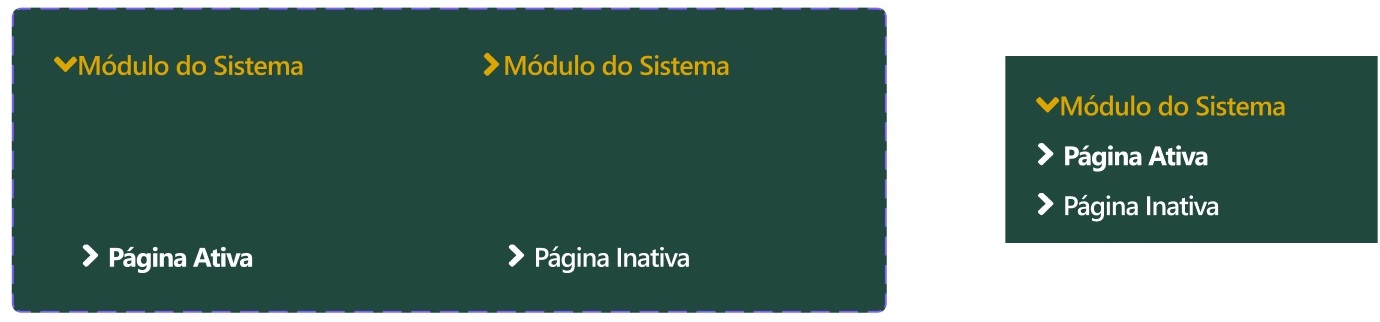
\includegraphics[width=\linewidth]{mastercomponent.jpg}
    \caption{Exemplo de Composição de elementos.}
    \label{fig:mastercomponent}
  \end{figure}

  \begin{citacao}[brazil]
    \begin{itemize}
      \item Atoms are the basic building blocks of all matter. Each chemical element has distinct properties, and they can’t be broken down further without losing their meaning. (Yes, it’s true atoms are composed of even smaller bits like protons, electrons, and neutrons, but atoms are the smallest functional unit.)
      \item Molecules are groups of two or more atoms held together by chemical bonds. These combinations of atoms take on their own unique properties, and become more tangible and operational than atoms.
      \item Organisms are assemblies of molecules functioning together as a unit. These relatively complex structures can range from single-celled organisms all the way up to incredibly sophisticated organisms like human beings.
    \end{itemize}
    \cite{atomic_design}
    \end{citacao}

  \begin{figure}[h!]
    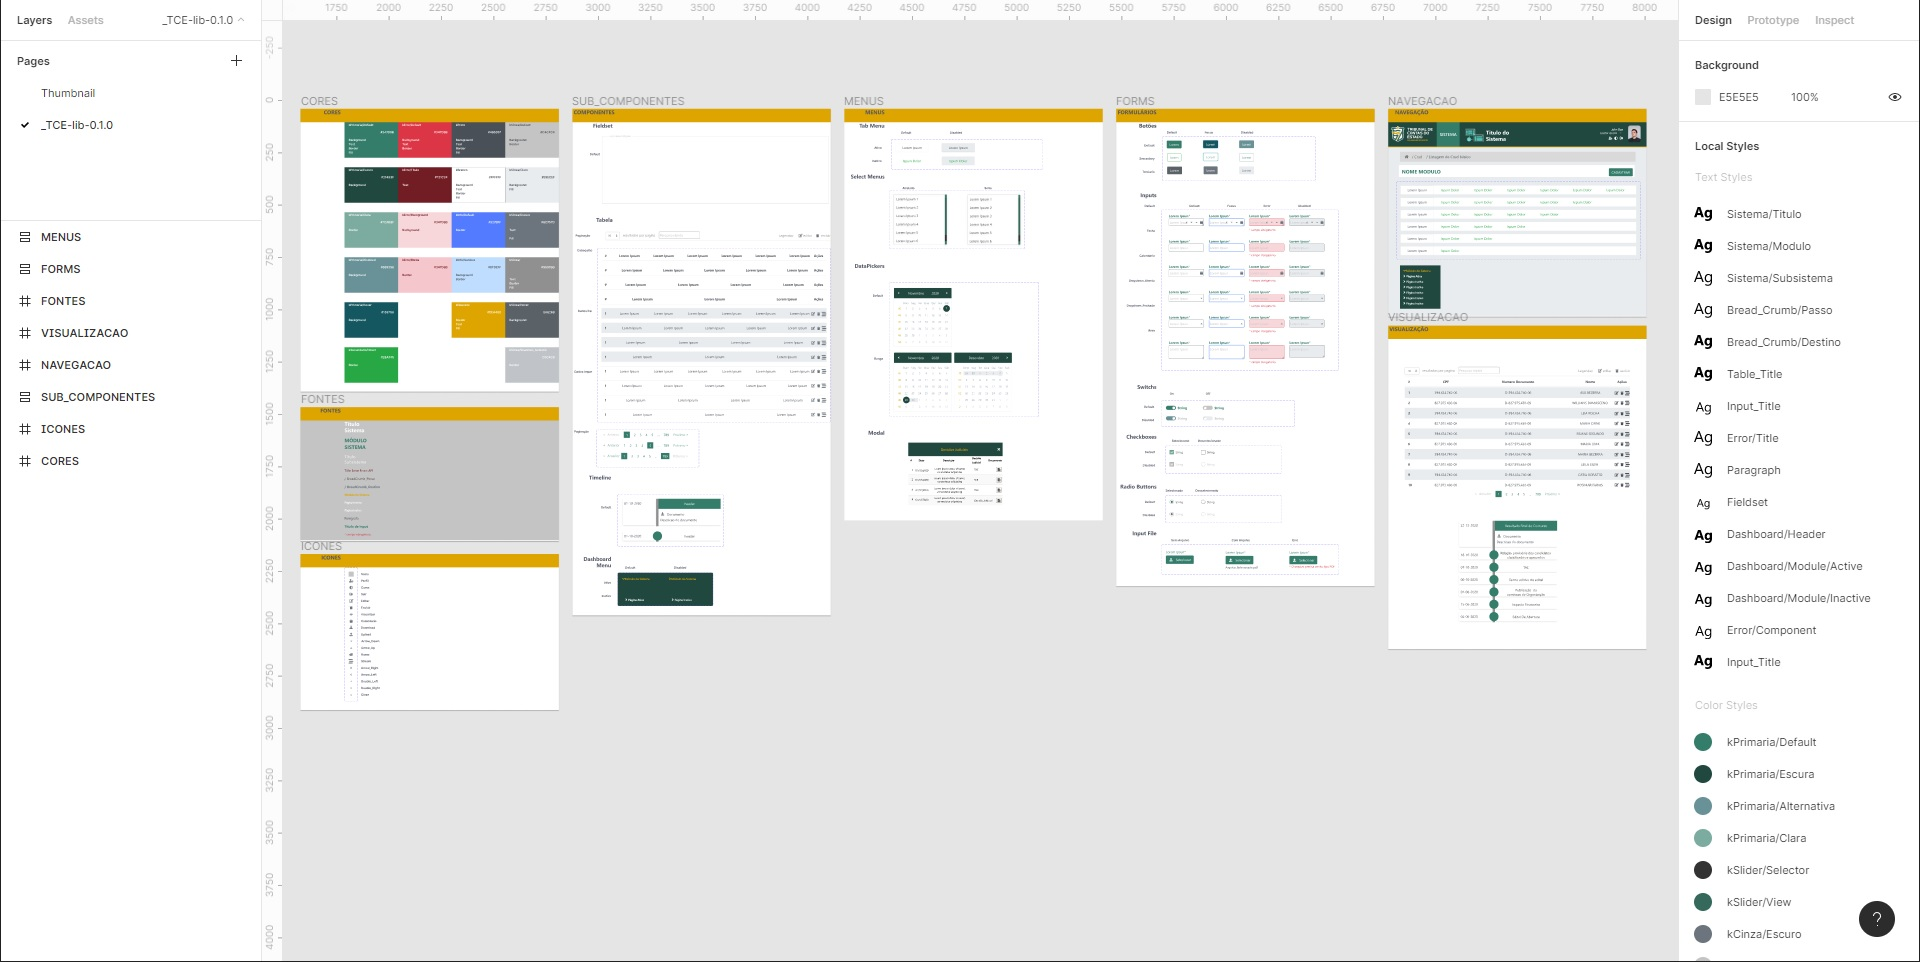
\includegraphics[width=\linewidth]{figma_010.jpg}
    \caption{Resultado Da primeira iteração do Figma.}
    \label{fig:tcenglib}
  \end{figure}

\section{Teste de Execução e Problemas Encontrados} \label{secao33}

  Após a criação do modelo existente o conjunto de compoentes criado com esse modelo foi utilizado para realizar a prototipação de um projeto de desenvolvimento de sistema em andamento no TCE-RN com o intuito de validar com o clientes, que era a Diretoria de Atos de Pessoal, as interfaces a serem concluidas junto com o sistema.

  Com a ajuda da bibliteca de componentes as telas do sistema foram criadas em algumas horas possuindo alta fidelidade e permitindo a experimentação dos clientes para testar os diferentes fluxos do sistema. Contudo por causa da cultura do tribunal os testes de usabilidade nao foram feitos de maneira extensiva e multiplas alterações foram solicitadas ou descobertas outras necessiaddes durante a etapa em que o desenvolvimento da aplicação havia sido iniciado. Essas alterações passaram por novas fazes de validação por meio de prototipagem e ocorreram de forma mais rápida do que o desenvolvolvimento tradicional em que as alterações seriam feitas diretamente na aplicação no front para serem testada e validadas junta ao cliente.

  Durante essas refatorações foram encontrados alguns problemas com a escolha da arquitetura da biblioteca. A separação dos componentens usando o modelo atomico por si só e a estrutura de separação adotada não tornava a biblioteca de componentes intuitiva de ser usada. A nomenclatura dos componentes tambem poderia ser melhorada de modo a favorer localização e facilitar o uso desses componentes.
  Por sua vez a biblioteca de componentes criadas pelo tribunal usando Angular tinha uma amplitude muito grande no gradiente de cinza e possuia elementos que poderiam apresentar confusão dependendo da sua prioridade e estados como botões terciarios habilitados e desabilitados que não comunicavam bem a sua função pois misturavam as tonalidades com seus estados secundarios.

  \begin{figure}[h!]
    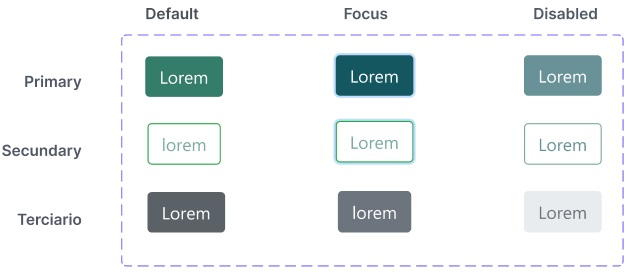
\includegraphics[width=\linewidth]{buttons_old.jpg}
    \caption{Diferentes estados de botões da biblioteca de compoentes do TCE-RN.}
    \label{fig:buttons_old}
  \end{figure}

\section{O Nascimento De Um Proto Sistema De Design} \label{secao34}

  A medida que se avançava o desenvolvimento deste trabalho e maior foi o contato com sistemas de design em estagios de desenvolvimento mais maduros ou consolidados como fonte de estudo e referencia, entao, notou-se que a complexidade e o esforço desprendido para a construção de um sistema de design mais abrangente, contendo não so uma biblioteca de componentes para prototipação mas tambem a sua implementação eram muito maiores do que eram possiveis obter da equipe dedicada a este trabalho. Surgiu então a ideia de se criar as diretrizes para a evolução da biblioteca de componentes atualmente existentes no TCE-RN, melhorando refinando o estilo dos elementos atualmente presentes para melhor comunicar a informação com os usuarios, diminuindo as variações existentes para obter biblioteca com maior conformidade.

  
  \begin{wrapfigure}{l}{0.5\textwidth}
    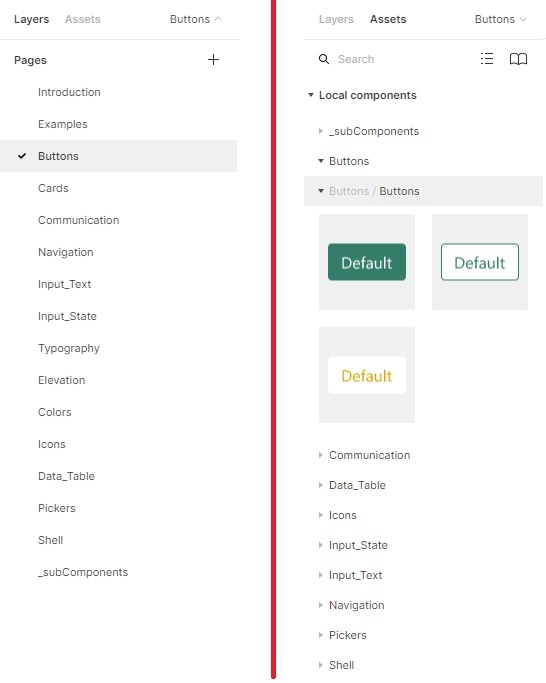
\includegraphics[width=\linewidth]{Component_Separation.jpg} 
    \caption{Separação dos Componentes }
    \label{fig:wrapfig}
  \end{wrapfigure}
  
  Os elementos adicionados no figma são classificados segundo a propria ferramenta como frames, groups e objects, enquanto os dois primeiros representam estruturas organizacionais o ultimo compreende um outro conjunto de elementos como por exemplo textos, formas e imagens. A associação desses elementos é usada para criar componentes, que são as entidades mais importantes do figma usadas para representar os items do nosso SD.

  Um arquivo do figma separa a estrutura de interação com os elementos em dois grandes grupos, layers, onde se encontram paginas que contem elementos que podem ser trabalhados, e assets, que contem apenas elementos mestres para importação em paginas na forma de instancias dos mestres. Em assets tem encontramos quais elementos estão disponiveis para serem exportados para a biblioteca de componentes.

  Chegar em uma boa estruturação dos componentes para exportação da biblioteca e viabilizar uma experiencia facil e intuitiva no desenvolvimento de prototipos é um dos objetivos principais desse trabalho e o modo com foi dividido se acredita ter chegado em um estado organizacional satisfatorio apesar da falta de testes de usabilidade extensivos.

  No fim valendo-se de uma funcionlidade do figma de tornar paginas com nomes iniciados com sublinhado proprias apenas para o uso interno projeto seguiu a seguinte estruturação: \underline{ }subComponents contem elementos herdados da arquitetura atomica inicialmente desenvolvida, esta pagina contem elementos que são fundamentalmente utilizados em outras estruturas e em tese não deveriam ter seus elementos subdivididos nem usados independentemente. Na sequência cada pagina contendo elementos em um frame respectivo a suas versões web sendo esses Buttons, Cards, Communication, Navigation, Input\underline{ }Text, Input\underline{ }State, Data\underline{ }Table, Pickers, Shell Colors, Typography, Icons.

  Adicionalmente uma pagina contendo exemplos de construção de telas foi adicionada a biblioteca para melhor guiar o desenvolvimento de templates por parte dos utilzadores do sistema de design assim como uma pagina introdutoria, contendo explicações sobre a separação do documento assim como os meios para utilizar a biblioteca. Por ultimo um pagina com um guia contendo os estilos e como aplicar diferentes elevações a elementos do front-end para inciar o desnevolvimento de elementos para dispositivos moveis.

  % Um arquivo do figma separa os elementos criados dentro do programa em dois grandes grupos Layers e Assets, estes elementos podem ser um frame ou grupo, usado para conter outros elementos assim como objetos unitarios adicionados ao canvas.

  % Separou-se os diversos grupos de elementos em paginas de modo a limitar o escopo dos itens incluidos em sub pastas nos assets para obter uma melhor granularidade no trabalho, e permitir o uso de 
  